\chapter*{Introduction}

Les systèmes biologiques qui nous entourent présentent une incroyable diversité de structures leur permettant d'évoluer et de s'adapter à leur environnement par l'échange, le stockage et le traitement d'information venant de ce dernier.
%Exemples ?
% Le blob est par exemple un être unicellulaire capable de s'étendre sur plusieurs mètres. Uniquement grâce aux communications chimiques opérant au sein de son plasmodium, il est capable de trouver le chemin le plus court dans un labyrinthe entre deux points sur lesquels sont placés de la nourriture \cite{Nakagaki2000IntelligenceMB} ou de retrouver une configuration optimale d'un réseau de transport. Ils sont même capables d'apprentissage~: deux entités qui fusionnent se transmettent des connaissances de leur environnement, montrant qu'elles ont chacune emmagasiné, à un point, de l'information sur ce dernier.
% Les colonies de fourmis, quant à elles constituées de milliers, voire de millions d'individus, sont capables de s'auto-organiser pour effectuer des tâches complexes de coopération pour construire leur nid, se défendre face aux prédateurs et trouver leur nourriture via une communication par leurs phéromones, son et toucher.
Autrement formulé, ces systèmes biologiques présentent des capacités de calcul remarquables, ce qui a inspiré de nombreux algorithmes d'optimisation en informatique, imitant par exemple les colonies de fourmis, les essaims d'abeilles, les groupes de chats, les bancs de poissons ou encore les baleines, tous ces groupes d'animaux présentant des méthodes de communication décentralisées efficaces pour accomplir une tâche donnée~\parencite{Darwish2018BioinspiredCA,nature_inspired_2020}.
Un parangon de système biologique de calcul est sans conteste le cerveau humain ou animal, qui est capable d'exécuter des tâches de calcul et surtout d'apprentissage incroyablement sophistiquées via une multitude de signaux électriques et chimiques circulant entre les neurones et au sein des vaisseaux sanguins.
L'inspiration biologique occupe ainsi une place de premier rang dans les débuts de la recherche en intelligence artificielle.
Les premiers modèles d'apprentissage automatique ont ainsi été développés en s'appuyant sur le modèle biologique du neurone, afin de chercher à imiter les capacités d'évolution et d'adaptation à l'origine de la notion d'apprentissage dans les réseaux de neurones biologiques. Le perceptron, modèle à l'origine des réseaux de Deep Learning les plus performants à l'heure actuelle, s'inspirait par exemple d'un modèle de neurone biologique~\parencite{McCulloch1990ALC}.
La diversité des applications actuelles de l'apprentissage automatique et le développement de nombreux modèles très performants ont amené la recherche en apprentissage automatique à se concentrer principalement sur une approche algorithmique et computationnelle de ces réseaux, en particulier pour les architectures de Deep Learning.
Cet éloignement de la biologie permet de s'extraire des contraintes physiques liées au neurone pour envisager des règles de calcul adaptées à des tâches spécifiques.
Néanmoins, la biologie, par sa diversité de comportements encore incompris, reste une source d'inspiration abondante pour apporter des paradigmes alternatifs ou complémentaires aux modèles d'apprentissage existants dans l'état de l'art. De plus, le comportement du cerveau est loin d'être entièrement compris et modélisé, ce qui signifie que les possibilités d'inspiration biologique sont constamment en train d'évoluer. Les réseaux de neurones impulsionnels (\emph{Spiking Neural Networks}) sont un exemple de modèle d'apprentissage illustrant une complémentarité récente entre l'approche bio-inspirée et l'approche computationnelle. Ces réseaux de neurones ont été développés dès les années 1990~\cite{Maass1996NetworksOS} et s'appuient directement sur le modèle biologique du neurone~; cependant, ils apparaissent dans de nombreux travaux récents comme une méthode montante dans le domaine de l'apprentissage automatique pour la conception de modèles d'apprentissage moins énergivores et distribués grâce à la conception d'architectures matérielles neuromorphiques telles que LOIHI \footnote{\url{https://www.intel.com/content/www/us/en/research/neuromorphic-computing.html}}. De nombreux travaux cherchent ainsi à adapter des réseaux de neurones classiques de l'état de l'art dans une version impulsionnelle, faisant ainsi passer les SNN de la biologie au calcul~\cite{Schuman2022OpportunitiesFN}.
%\cite{Yamazaki2022SpikingNN}.

L'inspiration biologique apporte ainsi de nouveaux paradigmes de calcul pouvant se combiner avec des approches plus appliquées. Nous pensons pour cette raison qu'il est pertinent de continuer à explorer des modèles d'apprentissage automatique inspirés de la biologie.
Dans cette thèse, nous voulons explorer la notion d'architecture modulaire. Cette propriété de modularité est partagée par de nombreux systèmes biologiques et artificiels et présente des avantages en termes de réutilisation, de robustesse aux fautes, de redondance et de traitement local de l'information \parencite{clune_evolutionary_2013}.
De nombreuses modélisations générales du cortex cérébral, telles que~\cite{binzegger05, Meunier2009HierarchicalMI,sporns_structure_2013,betzel_multi-scale_2017} proposent ainsi que le cortex est une architecture composée de modules auto-organisés. Ces modules communiquent autour des informations sensorielles collectées par l'organisme. Cette communication est réalisée de façon interne, liant des informations sensorielles et abstraites provenant de différentes parties du cortex et à différentes échelles spatiotemporelles. Enfin, bien qu'une hiérarchie de traitement de l'information apparaisse entre ces modules, certains traitant des entrées sensorielles et d'autres des entrées plus abstraites, de nombreux circuits de rétroactions entre les modules semblent présents à différents niveaux de l'architecture.
La recherche d'architectures cognitives s'inspirant de l'architecture du cortex cérébral est un enjeu de longue date dans la recherche en apprentissage automatique. Il s'agit de développer des réseaux de neurones autonomes, capables de mémoire et de prise de décision de façon non supervisée, qui s'inspirent des architectures modulaires présentes dans le cerveau humain et qui cherchent à imiter certains comportements \parencite{Kotseruba201840YO}. Le développement de la robotique appelle également à envisager des modèles d'apprentissage directement liés à la perception sensorielle, en s'inspirant des architectures modulaires existant dans le cortex et qui permettent le traitement de cette perception.
% Notons que notre démarche se veut d'inspiration biologique, tout en restant dans le domaine de l'informatique.
% Les notions biologiques que nous considérons restent des constats généraux, que nous voulons implémenter dans une démarche de création de système d'apprentissage informatique. 

Outre l'inspiration biologique liée à la structure corticale, la construction de systèmes d'apprentissage modulaires découle également d'une motivation computationnelle.
La modularité en informatique prend de nombreuses significations.
Nous entendons ici par système modulaire un système de calcul composé d'une multiplicité de sous-structures interchangeables qui interagissent entre elles par le biais d'interfaces définies. 
Dans une architecture modulaire, ces sous-structures communiquent de façon locale, sans être supervisées par un processus externe.
Nous pensons que cette approche modulaire est propice à faire émerger des nouveaux paradigmes d'apprentissage au sein d'architectures neuronales. 
En effet, la combinaison de principes et d'algorithmes simples en architecture modulaire peut mener au développement de mécanismes de calcul complexes au sein du système. De ce fait, nous pensons que cette approche est pertinente pour la conception de systèmes innovants et robustes.
Ces mécanismes de calcul complexes mènent à des comportements émergents, c'est-à-dire que le comportement global du système résulte bien de l'interaction entre les modules et non seulement de la somme des comportements des modules pris individuellement~: il s'agit de systèmes complexes.

Ces sous-structures, les modules, peuvent avoir un rôle et une structure différentes, spécifiquement concue pour une tâche ; ex brooks. 
On peut imaginer des modules de structures similaires, mais dont les paramètres ont été prédéfinis : ex DNF. Enfin, la notion de module que nous voulons explorer est celle de modules interchangeables, de même structure, et dont le rôle dans l'architecture va se différencier par apprentissage.
Par exemple, \cite{brooks_sumsumption_85} construit une architecture robotique composée de modules comportementaux simples, tels que "marcher", "regarder", qui interagissent entre eux. Il montre que l'interaction de tous ces comportements de base permet au système de réagir de manière autonome à son environnement. L'intelligence d'essaim est un autre exemple de système modulaire exhibant des mécaniques d'apprentissage complexe via l'interaction entre des agents simples \parencite{Bonabeau1999SwarmI}.

Dans la démarche d'explorer un modèle d'apprentissage informatique inspiré de l'architecture modulaire du cortex, nous proposons dans cette thèse de construire une architecture de cartes auto-organisatrices de Kohonen.
Les cartes de Kohonen \parencite{Kohonen1982} sont un exemple de modèle d'apprentissage initialement inspiré de considérations biologiques.
Ces modèles sont caractérisés par leur capacité à représenter des données de façon ordonnée sur un espace de dimension plus faible (typiquement une ou deux dimensions). Cette organisation topographique des données se forme à l'issue d'un processus d'apprentissage, d'où le concept d'auto-organisation.
Les cartes de Kohonen sont initialement inspirées des cartes topographiques présentes dans les cortex sensoriels ou moteurs, et présentent des similarités avec ces derniers dans leur organisation finale.
Les mécanismes de mise à jour des poids, d'abord calculés grâce à des champs récepteurs directement inspirés de la biologie, ont ensuite évolué vers des règles plus computationnelles de calcul de distance entre les entrées et les poids des cartes.
La littérature autour des cartes de Kohonen, bien qu'extensive, s'est principalement attachée à leur utilisation dans des tâches de classification, de clustering ou de compression de données~; les développements de ce modèle se sont également attelés à l'augmentation des performances des cartes pour sur des applications d'apprentissage automatique et de fouille de données~\parencite{kohonen_essentials_2013}.
Nous pensons que leur inspiration biologique, leurs propriétés d'organisation et de représentation en deux dimensions d'un espace complexe et la simplicité de leurs règles de mise à jour en font des candidates naturelles pour la création d'une architecture modulaire d'apprentissage.

Cette idée d'architecture modulaire de cartes n'est pas nouvelle et est d'ailleurs formulée par Kohonen dès 1995~:
\begin{quote}
Un objectif à long terme de l'auto-organisation est de créer des systèmes autonomes dont les éléments se contrôlent mutuellement et apprennent les uns des autres. De tels éléments de contrôle peuvent être implémentés par des SOMs spécifiques~; le problème principal est alors l'interface, en particulier la mise à l'échelle automatique des signaux d'interconnexion entre les modules et la collecte de signaux pertinents comme interface entre les modules. Nous laisserons cette idée aux recherches futures.
Traduit de \cite{Kohonen1995SelfOrganizingM}
\end{quote}

Depuis, bien que des travaux aient proposé des architectures de carte auto-organisatrices, peu ont effectivement exploré l'aspect topographiquement ordonné et la simplicité des règles mise à jour des poids d'une carte pour les assembler en architectures modulaires comportant des rétroactions~: des architectures non-hiérarchiques.
C'est pourquoi nous nous intéressons à cet aspect dans cette thèse.
% L'objectif des travaux que nous présentons est alors de proposer un modèle de carte qui puisse être utilisée en tant que module, de définir l'interface entre les modules afin de créer une architecture, et de comprendre les comportements de calcul qui émergent de l'association des modules, dans un but à long terme de création d'une architecture modulaire non-hiérarchique de cartes auto-organisatrices.

% Finalement, la conception d'une architecture modulaire d'apprentissage s'inspire d'une part des propriétés de modularité et d'émergence observées dans différents systèmes naturels en particulier dans le cerveau, et artificiels comme l'intelligence d'essaim ou les réseaux de neurones profonds.
% La propriété de modularité permettrait à une architecture de réaliser des calculs complexes en exploitant la collaboration et l'interaction des modules de façon décentralisée.
% Dans cette démarche, les SOMs sont de bonnes candidates pour être associés en architectures modulaires. Elles sont en effet inspirées de l'organisation des aires corticales, aires qui sont associées dans le cerveau en architecture modulaires. L'introduction de rétroactions dans ces architectures permettra de plus d'explorer de nouveaux comportements computationnels.
L'approche que nous avons privilégiée pour la construction d'une telle architecture est synthétique~: nous définissons un modèle en s'appuyant sur l'état de l'art et les travaux précédents, puis nous cherchons à évaluer son comportement, afin de guider les améliorations ou applications qui en découlent. Nous proposons dans cette thèse un modèle d'architecture de cartes auto-organisatrices~: CxSOM.
L'objectif de la thèse est de fournir un cadre méthodologique visant à comprendre et observer les mécanismes d'apprentissage émergeant des règles de calcul que nous avons définies.

La notion d'architecture cognitive présentée plus haut cherche à explorer de grands principes liés à la cognition tels que l'apprentissage autonome, sans supervision, le traitement de données temporelles, l'apprentissage sur le long terme sans oubli catastrophique des données précédentes et la fusion de données multimodales, s'inspirant du traitement multisensoriel du cerveau humain.
L'architecture que nous proposons, par sa conception, vise à long terme l'application à de telles tâches. Cette problématique étant très vaste, nous avons choisi dans cette thèse de nous concentrer sur la tâche particulière d'apprentissage associatif de données multimodales. 
Il s'agit d'apprendre des relations existant entre des entrées provenant de différentes modalités, en plaçant cet apprentissage de relations à un niveau interne à l'architecture et non en combinant les entrées. Le but est d'apprendre une représentation des entrées, mais également de leurs relations.
Dans cette optique d'apprentissage de représentation de relations entre entrées, nous proposerons des outils de visualisation et des indicateurs permettant de comprendre ces mécanismes.

 \begin{center}
    \fbox{
    \parbox{0.7\textwidth}{En résumé, cette thèse vise à répondre à deux problématiques principales entremêlées~: proposer une nouvelle architecture non-hiérarchique de cartes auto-organisatrices exploitant totalement l'aspect topographiquement ordonné de ce modèle d'apprentissage, et étudier comment mettre en évidence et évaluer l'apprentissage associatif qui émerge d'une telle architecture.}
 }
 


\begin{figure*}[h!]
    \vspace{1cm}
    \centering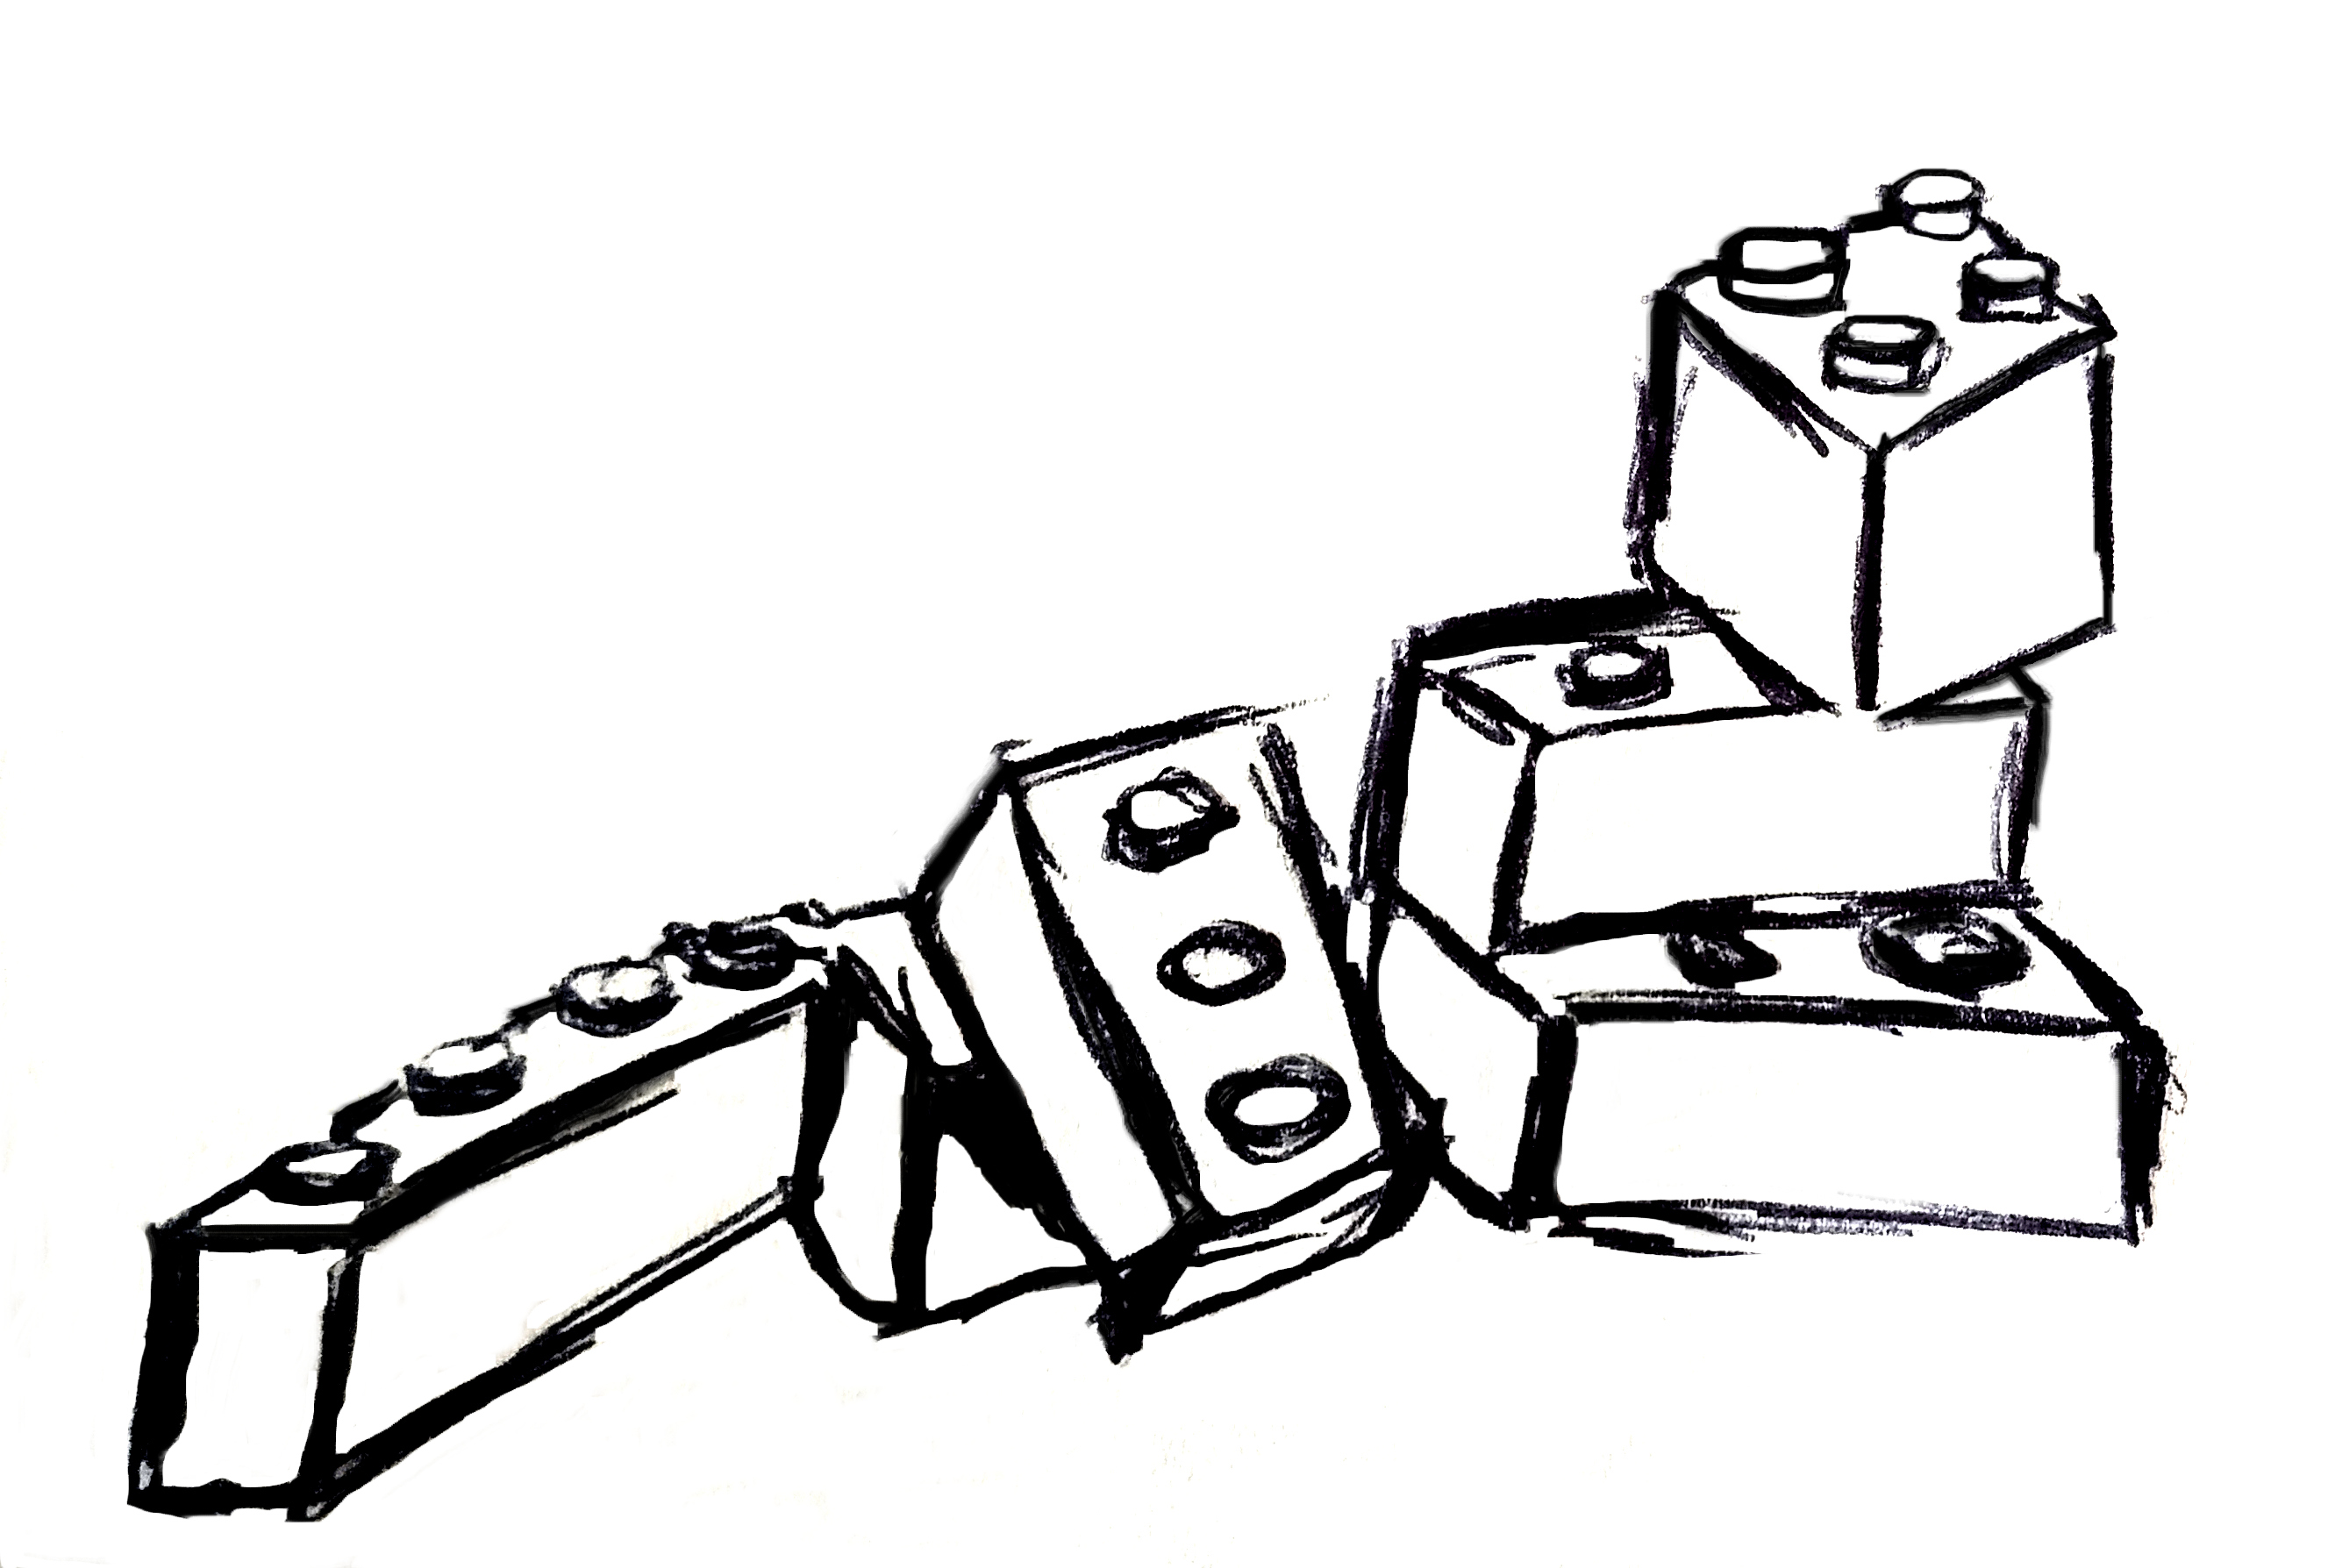
\includegraphics[width=0.2\textwidth]{lego2.jpg}
    \vspace{1cm}
\end{figure*}
\end{center}

Le manuscrit est organisé de la façon suivante.
Le chapitre~\ref{chap:architectures} présente un état de l'art des architectures de cartes auto-organisatrices existantes dans la littérature. Ces modèles d'architectures sont issus de plusieurs domaines, de l'apprentissage automatique aux neurosciences computationnelles.
Le chapitre propose une revue des modèles principaux en s'attachant à unifier les notations et leurs désignations afin d'identifier les points communs et différences principales de conception de ces modèles.
Cet état de l'art nous permettra de situer le modèle que nous proposons au regard de la littérature existante.

Nous détaillerons ensuite le modèle d'architecture décentralisée de cartes auto-organisatrices que nous proposons dans cette thèse, que nous avons appelé CxSOM, pour \emph{Consensus-driven Multi-SOM}. 
Nous définissons un modèle de carte qui peut être assemblé à volonté en architecture non-hiérarchiques.
Dans ce modèle, les activités des différentes cartes sont interdépendantes et l'apprentissage s'appuie sur une recherche de consensus entre les cartes pour la recherche d'un BMU.
Nous présenterons ce modèle au chapitre~\ref{chap:modele}. Le chapitre~\ref{chap:relaxation} s'attarde ensuite sur une analyse plus approfondie de la recherche de consensus constituant l'interface entre les cartes afin de valider ce mécanisme en tant qu'algorithme de choix de BMU pour l'apprentissage.

Si notre approche synthétique a pour but à long terme de concevoir une architecture comportant de nombreux modules ainsi que des connexions temporelles, nous avons concentré cette thèse sur l'analyse expérimentale des comportements d'apprentissage dans des architectures de deux et trois cartes.
Le pari de l'approche synthétique est de faire émerger des nouveaux comportements, aussi faut-il pouvoir les mettre en évidence. Nos travaux se sont alors vite confrontés à une difficulté de visualisation d'une telle architecture de cartes. 
Cette thèse appuie donc une méthodologie d'analyse expérimentale de l'architecture modulaire, ce qui nous permettra d'en tirer des comportements élémentaires qui serviront à poser les jalons de la construction d'une architecture plus complexes.
Nous introduisons au chapitre \ref{chap:repr} cette méthode expérimentale et un cadre de représentation des entrées, et questionnons les représentations exprimant comment une architecture de cartes encode les entrées et leurs relations.
Nous présentons ensuite au chapitre \ref{chap:analyse} les comportements élémentaires d'apprentissage associatif observés sur des architectures de deux et trois cartes en une dimension, à partir des représentations que nous avons proposées. Nous présenterons en particulier un comportement de prédiction d'entrée rendu possible par les rétroactions présentes dans le modèle d'architecture.
Nous explorons au chapitre~\ref{chap:indicateur} des indicateurs numériques originaux d'évaluation de l'apprentissage associatif par l'architecture de cartes, dans le but d'étendre l'analyse du modèle à des architectures plus grandes, qui seraient difficilement représentables graphiquement.
Le chapitre \ref{chap:analyse2D} étend enfin les mécanismes d'apprentissage que nous avons identifé à des architectures de cartes en deux dimensions, se plaçant comme une étude préliminaire pour saisir la scalabilité du modèle.




% Idées : plutôt se concentrer sur la SOM en elle-même. Champs d'application, performances, remarquer que les SOM ont des performances pour extraire des représentations, inspi biologique
% Voila ce qui n'a pas été réalisé, et voila ce que je propose : injecter de l'information de position 
% démarche synthétique
% caractériser le comportement émergent des cartes.



% Des systèmes en apparence simples présentent ainsi des capacités d'optimisation de tâches. Le blob est par exemple un être unicellulaire capable de s'étendre sur plusieurs mètres. Uniquement grâce aux communications chimiques opérant au sein de son plasmodium, il est capable de trouver le chemin le plus court dans un labyrinthe entre deux points sur lesquels sont placés de la nourriture \cite{Nakagaki2000IntelligenceMB} ou de retrouver une configuration optimale d'un réseau de transport. Il sont même capables d'apprentissage~: deux entités qui fusionnent se transmettent des connaissances de leur environnement, montrant qu'elles ont chacune emmagasiné, à un point, de l'information sur ce dernier.
% Les colonies de fourmis, quant à elles constituées de milliers, voire de millions d'individus, sont capables de s'auto-organiser pour effectuer des tâches complexes de coopération pour construire leur nid, se défendre face aux prédateurs et trouver leur nourriture via une communication par leurs phéromones, son et toucher.
% Autrement dit, ces systèmes biologiques présentent des capacités de calcul remarquables. 
% Toutes ces stratégies mises en place par des systèmes biologiques ont inspiré de nombreux algorithmes d'optimisation imitant par exemple les colonies de fourmis, les essaims d'abeilles, les groupes de chats, les bancs de poissons ou encore les baleines, tous ces groupes d'animaux présentant des méthodes de communication décentralisées efficaces pour accomplir une tâche donnée~\cite{Darwish2018BioinspiredCA}.




% Les réseaux de neurones impulsionnels (\emph{Spiking Neural Networks}) sont un exemple de modèle d'apprentissage illustrant une complémentarité récente entre l'approche bio-inspirée et l'approche computationnelle.
% Ces réseaux de neurones ont été développés dès les années 1990~\cite{Maass1996NetworksOS} et s'appuient directement sur le modèle biologique du neurone.
% Ils apparaissent dans de nombreux travaux récents comme une méthode montante dans le domaine de l'apprentissage automatique pour la conception de modèles d'apprentissage moins énergivores et distribués, grâce à la conception d'architectures matérielles neuromorphiques telles que LOIHI \footnote{\url{https://www.intel.com/content/www/us/en/research/neuromorphic-computing.html}}. De nombreux travaux cherchent ainsi à adapter des réseaux de neurones classiques de l'état de l'art dans une version impulsionnelle, faisant ainsi passer les SNN de la biologie au calcul~\cite{Schuman2022OpportunitiesFN}.
% De tels modèles apportent de nouveaux paradigmes de calcul pouvant se combiner avec des approches plus appliquées.
% Nous pensons ainsi qu'il est pertinent de continuer à explorer des modèles d'apprentissage automatique inspirés de la biologie.